\begin{titlepage}
\begin{center}

% Upper part of the page. The '~' is needed because \\
% only works if a paragraph has started.

\includegraphics[width=0.35\textwidth]{./logo/ddmore_logo}~\\[1cm]

%\textsc{\LARGE }\\[1.5cm]
%
\textsc{\Large Technical Report}\\[0.5cm]

% Title
\HRule \\[0.4cm]
{ \huge \bfseries PK Macros in PharmML 0.6 \\[0.4cm] }

\HRule \\[1.5cm]


% Authors
\begin{minipage}{0.9\textwidth}
\begin{flushleft} \large
Maciej J \textsc{Swat}$^1$, Sarala \textsc{Wimalaratne}$^1$, Niels Rode \textsc{Kristensen}$^2$,\\
Roberto \textsc{Bizzotto}$^3$, Marc \textsc{Lavielle}$^4$ \\
\end{flushleft}
\end{minipage}
\bigskip


\begin{minipage}{0.9\textwidth}
\begin{flushleft} \large
$^1$\emph{EMBL - European Bioinformatics Institute, Cambridge, UK}, \\ 
$^2$\emph{Novo Nordisk A/S, Bagsv\ae rd, Denmark}, \\
$^3$\emph{National Research Council, Institute of Neuroscience, Padova, Italy}, \\
$^4$\emph{Inria Saclay, France}
\end{flushleft}
\end{minipage}


\vfill
\begin{figure}[htb]
\centering
  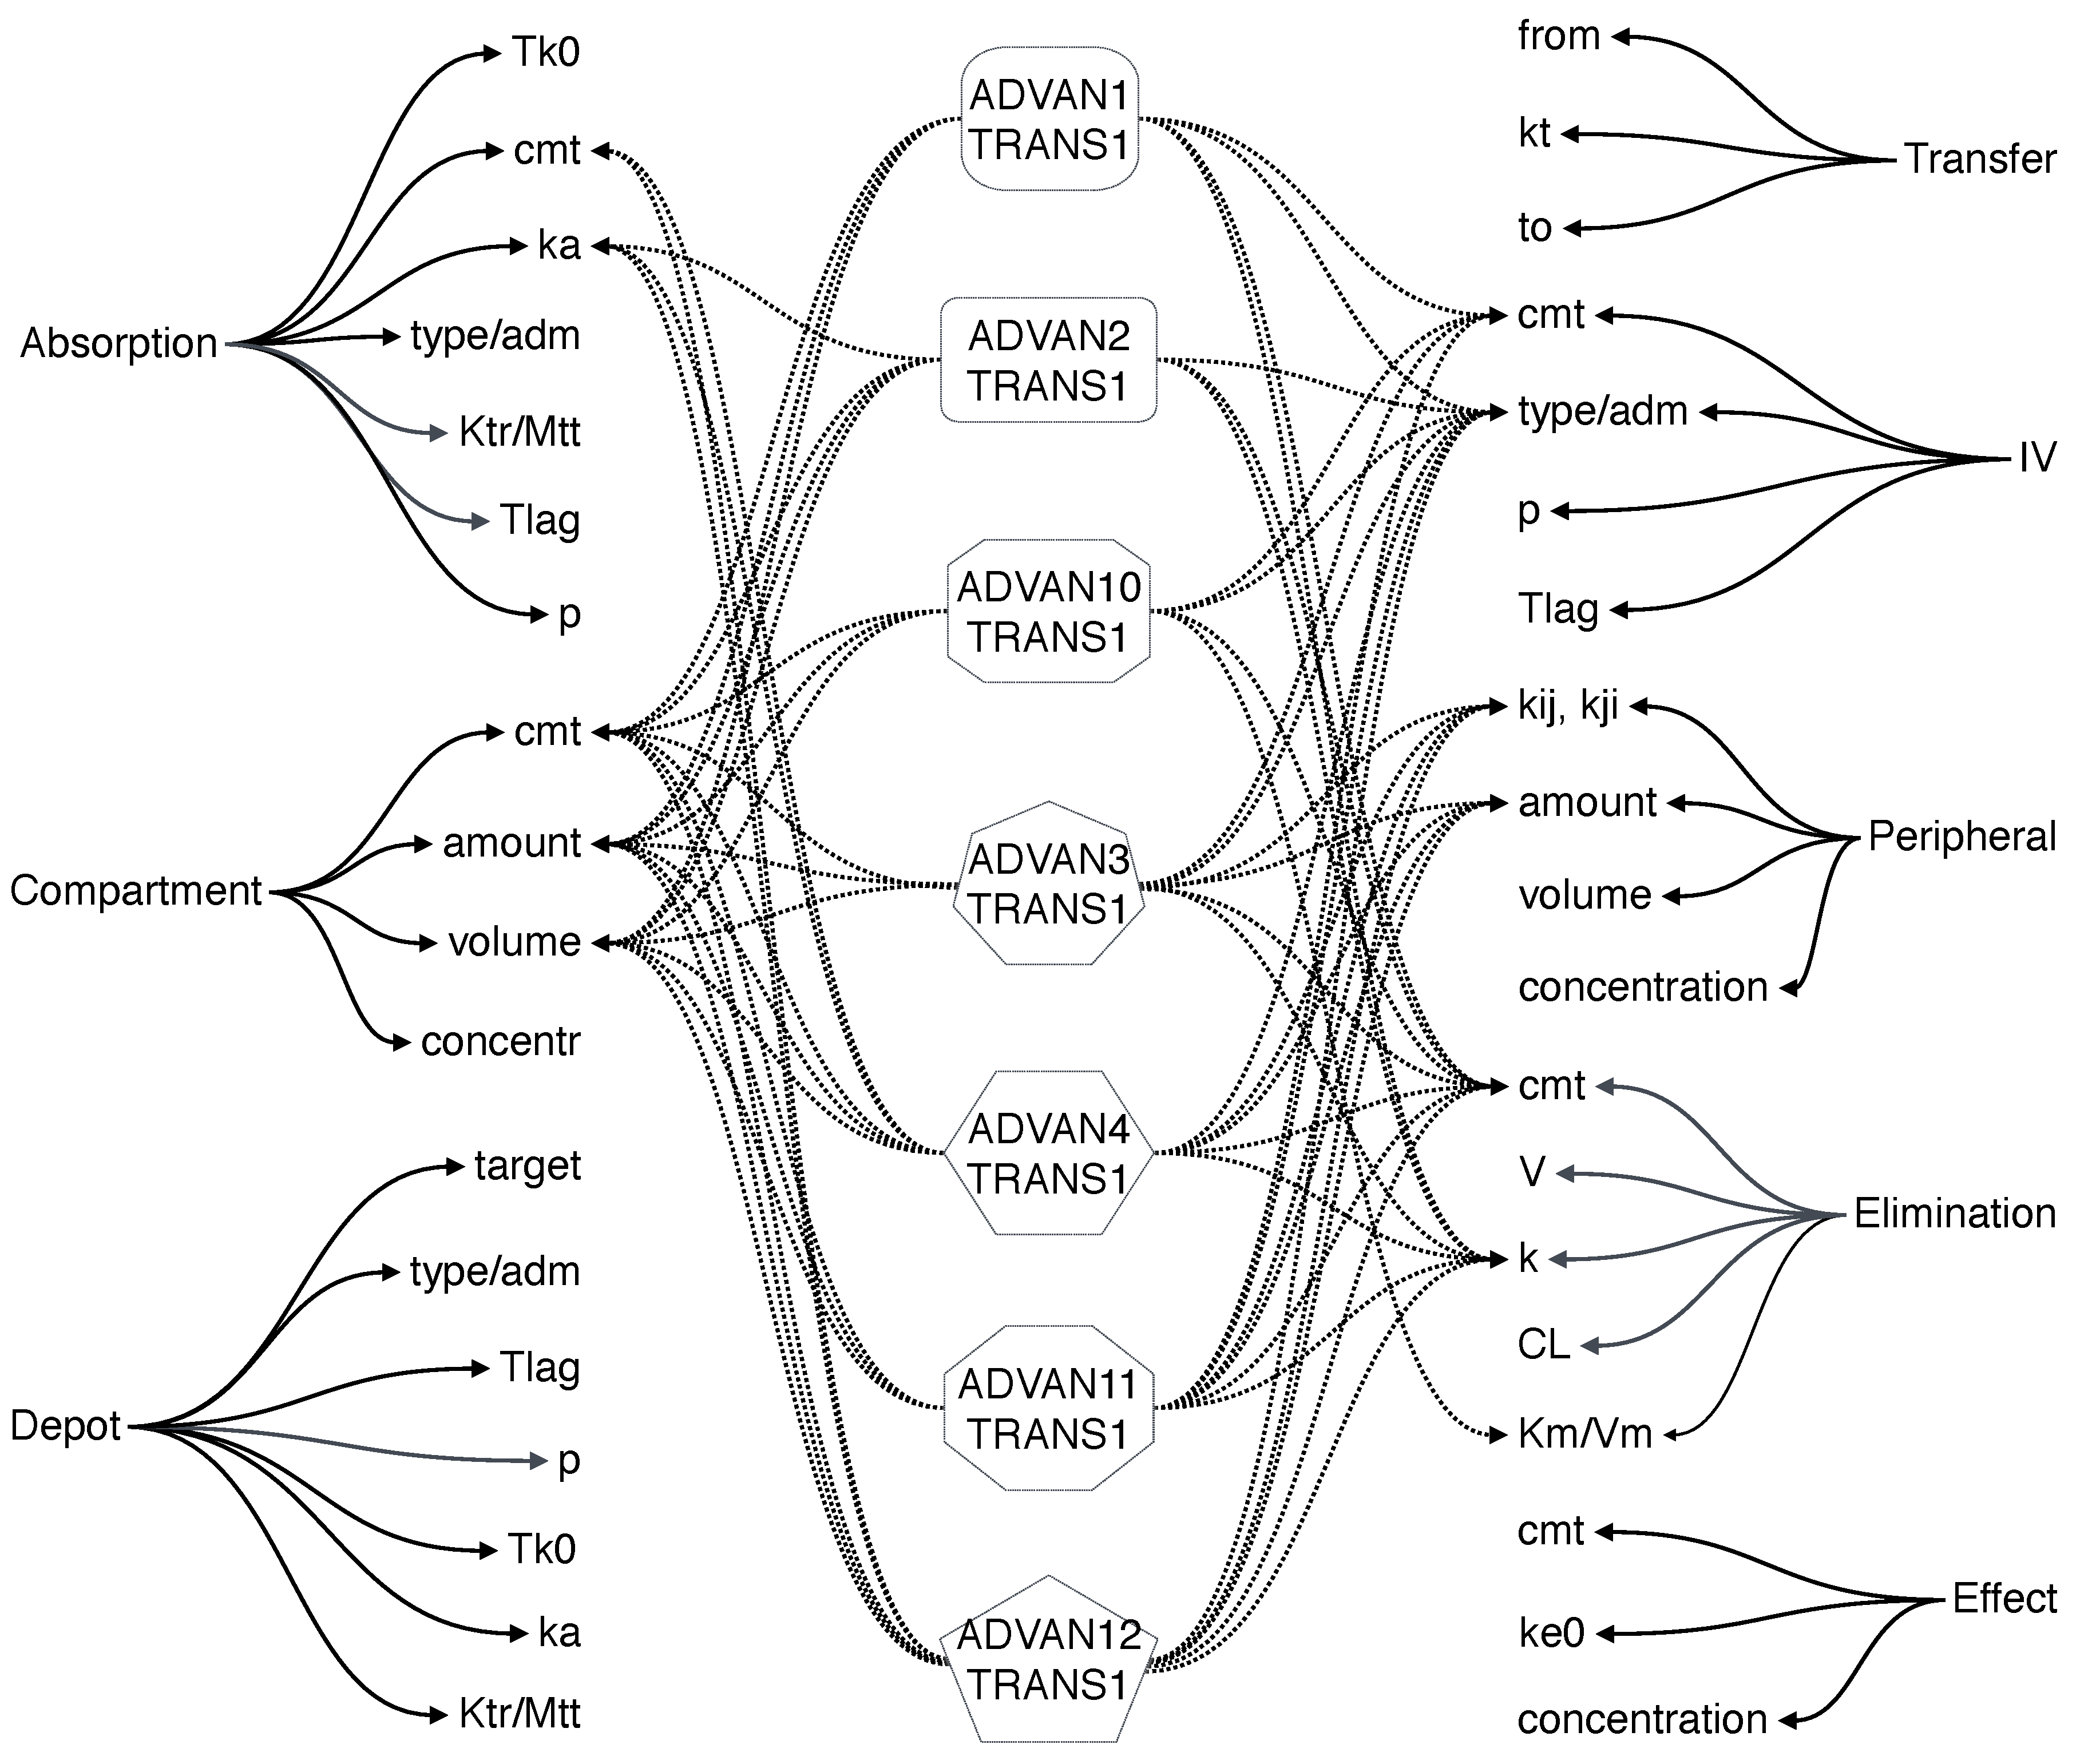
\includegraphics[width=0.70\linewidth]{pics/AdvanMacrosMaster.pdf}
\end{figure}

\vfill

% Bottom of the page
{\large \today \\}

\end{center}
\end{titlepage}